\section{Formalization}
\label{sec:formalization}
Given a state space $U$, a transition system $(I,T)$ consists of an
initial state predicate $I : U \to \bool$ and a transition step
predicate $T : U \times U \to \bool$.
We define the notion of
reachability for $(I, T)$ as the smallest predicate $\reach : U \to
\bool$ which satisfies the following formulas:
\begin{gather*}
  \forall u.~ I(u) \Rightarrow \reach(u) \\
  \forall u, u'.~ \reach(u) \land T(u, u') \Rightarrow \reach(u')
\end{gather*}
A safety property $P : U \to \bool$ is a state predicate. A safety
property $P$ holds on a transition system $(I, T)$ if it holds on all
reachable states, i.e., $\forall u.~ \reach(u) \Rightarrow P(u)$,
written as $\reach \Rightarrow P$ for short. When this is the case, we
write $(I, T)\vdash P$. We assume the transition relation has the structure of a top level conjunction. Given $T(u, u') = T_1(u,u') \land \cdots T_n(u,u')$ we will write $T = \land_{i=1..n}$ for short. By further abuse of notation, $T$ is identified with the set of its top-level conjuncts. Thus, $T_i \in T$ means that $T_i$ is a top-level conjunct of $T$, and $S\subseteq T$ means all top level conjuncts of $S$ are top-level conjuncts of $T$. When a top-level conjunct $T_i$ is removed from $T$, we write $T \setminus \{T_i\}$

The set of all nominal guarantees of the system $G$ consists of conjunctive constraints $g \in G$. Given no faults (i.e., nominal system) and a transition relation $T$ consisting of conjunctive constraints $T_i$ as defined in section~\ref{sec:prelim}, each $g$ is one of the transition constraints $T_i$ where:

\begin{gather}
T = g_1 \land  g_2 \land \cdots \land g_n
\label{eq:Tn}
\end{gather}

We consider an arbitrary layer of analysis of the architecture and assume the property holds of the nominal relation $(I,T) \vdash P$. Given that our focus is on safety analysis in the presence of faults, let the set of all faults in the system be  denoted as $F$. A fault $f \in F$ is a deviation from the normal constraint imposed by a guarantee. Without loss of generality, we associate a single fault and an associated fault probability with a guarantee. Each fault $f_i$ is associated with an \emph{activation literal}, $\mathit{af}_i$, that determines whether the fault is active or inactive. %Any ``faults" in a mid-layer are simply violated guarantees, or deviations from normal behavior. 

%The faults in the safety annex are defined on leaf level components. Thus, for the lowest analysis layer, we must take into consideration faults and the guarantees their activation may violate. A fault $f \in F$ is a deviation from the normal constraint imposed by a guarantee. For the purposes of this paper, each guarantee at the leaf layer of analysis has an associated fault. 

To consider the system in the presence of faults, consider a set $GF$ of modified guarantees in the presence of faults and let a mapping be defined from activation literals $\mathit{af}_i \in AF$ to these modified guarantees $\mathit{gf}_i \in GF$. 
\begin{center}
$\mathit{gf}_i =$ \textit{if} $\mathit{af}_i$ \textit{then} $f_i$ \textit{else} $g_i$\\
\label{eq:sigma}
\end{center}

The transition system is composed of the set of modified guarantees $GF$ and a set of conjunctions assigning each of the activation literals $\mathit{af}_i \in AF$ to false: 

\begin{gather}
T' = \mathit{gf}_1 \land \mathit{gf}_2 \land \cdots \land \mathit{gf}_n \land \neg \mathit{af}_1 \land \neg \mathit{af}_2 \land \cdots \land \neg \mathit{af}_n
\label{eq:T}
\end{gather}

\begin{theorem} If $(I,T) \vdash P$ for $T$ defined in equation~\ref{eq:Tn}, then $(I,T') \vdash P$ for $T'$ defined in equation~\ref{eq:T}.
\begin{proof}
By the mapping of each constrained activation literal $\neg \mathit{af}_i$ to the associated guarantee $g_i$ and the weakening of the antecedent by introduction of the activation literals, the result is immediate.
\end{proof}
\end{theorem}

Consider the elements of $T$ as a set $GF \cup AF$, where $GF$ are the potentially faulty guarantees and $AF$ consists of the activation literals that determine whether a guarantee is faulty. This is a set that is considered by an SMT solver for satisfiability during the model checking engine procedures. 

Given the extended transition system $T'$, if the $\mathit{af}_i \in \mathit{AF}$ are unconstrained and this causes violation of $P$, a counterexample is returned. For each counterexample, we can partition $\mathit{AF}$ into two sets which we call {\em non-faulty variables (NFV)} and {\em faulty variables (FV)}.  The set $\mathit{NFV}$ consists of a set of variables that are constrained to be false throughout the counterexample, and $\mathit{FV}$ contains those that can be non-deterministically assigned at some point in the trace. By mapping some of the variables in $\mathit{AF}$ to false, we know that associated guarantees in $\mathit{GF}$ are non-faulty for all considered executions. We define $T'(\mathit{NFV})$ as a relaxation of $T'$:

\begin{gather*}
T'(\mathit{NFV}) = \mathit{gf}_1 \land \mathit{gf}_2 \land \cdots \land \mathit{gf}_n \land \bigwedge \{\neg \mathit{af}_i | \mathit{af}_i \in \mathit{NFV} \}
\end{gather*}

The activation literals constrained to be false in $\mathit{NFV}$ cause their associated guarantees to be valid. When $\mathit{af}_i \in \mathit{AF}$ are given a true valuation (and thus are in $\mathit{NF}$), the associated guarantee will be violated. This violation causes the output that the guarantee constrains to become non-deterministic. The Boolean variables in $\mathit{FV}$ correspond to Boolean variables in the fault tree. 

%Given the extended transition system in Equation~\ref{eq:T}, if the $\mathit{af}_i \in \mathit{AF}$ are unconstrained and this causes violation of $P$, a counterexample is returned.  This counterexample is a partition of guarantees $\mathit{GF}$ into disjoint sets:  $\mathit{GF} = \mathit{NFV} \cup \mathit{FV}$. The set $\mathit{NFV}$ consists of nonfaulty variables: the associated $\mathit{af}_i$ are mapped to {\em false} in the counterexample, and the set $\mathit{FV}$ consists of faulty variables: the associated $\mathit{af}_i$ are mapped to {\em true} in the counterexample. In the remainder of this section, we assume that all $\mathit{af}_i \in \mathit{AF}$ are nondeterministically unconstrained and when active, cause the associated guarantee to be violated. Thus the output that the guarantee constrains becomes nondeterministic when the associated $\mathit{af}_i$ is true.


%%						DEFINE FT/FF
\begin{definition}
A fault tree $\mathit{FT}$ is a pair $(r, \mathcal{L})$ where:
\begin{itemize}
\item[] $r$: the root is a guarantee $r \in P$ corresponding to a violated property
\item[] $\mathcal{L}$: a Boolean equation containing faulty vars $\mathcal{L} \subseteq \mathit{FV}$
\end{itemize}
%The fault tree $\mathit{FT}$ is a Boolean equation in disjunctive normal form (DNF): $(r, \mathcal{L}) = r \lor \mathcal{L} = r \lor C_1 \lor \cdots \lor C_n$ for conjunctions $C_i$. 
\end{definition}

The terms $\mathit{af}$  in the Boolean formula $\mathcal{L}$ may be extracted as the set of leaf nodes of the fault tree. 

\begin{definition} 
A fault tree $FT = (r, \mathcal{L})$ is valid if and only if $(r, \mathcal{L})$ is satisfiable with a true valuation for $r$ and for all $\mathit{af} \in \mathcal{L}$. 
\label{def:validFT}
\end{definition}


Each layer of the architecture may contain multiple properties $P$. The subset $\pi$ of $P$ are the properties which have an associated fault tree and are either top level safety properties themselves or are used to prove the properties of a parent level. Due to this multiplicity, we do not compose single fault trees per layer, but rather forests of trees.

\begin{definition}
A fault forest $\mathit{FF}$ is a set of fault trees.
\end{definition}

\begin{definition}
A fault forest $\mathit{FF}$ is valid if and only if for all $\mathit{FT} \in \mathit{FF}$, $\mathit{FT}$ is valid.
\label{def:validFF}
\end{definition}


% 					COMPOSE FAULT FORESTS:
%%%%%%%%%%%%%%%%
%Let $n$ be the number of properties for some parent component $p$ and let $m$ be the number of properties for some child component $c$. Then the fault forest $\mathit{FF}_c$ is a mapping $\mathit{FF}_c : S_1 \rightarrow B$ for $S_1 = \{1,2,\dots,m\}$ and the set of Boolean equations $B$ and $\mathit{FF}_p: S_2 \rightarrow B$ for $S_2 = \{1,2,\dots n\}$. We use the notation $\mathit{seq(B)}$ to describe a sequence of Boolean equations.
%%%%%%%%%%%%%%%%%%%%%

%							SET UP FOR COMPONENT DEFINITION
A counterexample is a trace. That trace is a valuation that splits $\mathit{AF}$ into disjoint sets $\mathit{NFV} \cup \mathit{FV}$. Each counterexample determines a set $\mathit{FV}$ with respect to a property $\pi_i \in \pi$. This defines an associated fault tree $\mathit{FT}_i \in \mathit{FF}$ where the root of the tree is the property $\pi_i$.  

On the other hand, we also want to describe the non-faulty variables that are required for the proof of all $\pi_i \in \pi$ in order to have a valid component throughout composition. These are used in the relaxation of $T'$ and can be stated as $(I, T'(\mathit{NFV})) \vdash \pi$. A valid component has the potential to either prove pertinent properties (non-faulty variables) or violate properties (faulty variables), depending on the valuation of activation literals. 

%%					DEFINE COMPONENT
\begin{definition}
A component is the tuple $\mathit{Comp}(M, \mathit{FF}, \mathit{NFV}, \pi)$ where:
\begin{itemize}[label=\textbullet]
\item $M$: the model consisting of the set of child properties $P_c$ extended with non-deterministic faults: $\mathit{gf}_i \in P_c$ where $\mathit{gf}_i =$ \textit{if} $\mathit{af}_i$ \textit{then} $\mathit{f}_i$ \textit{else} $g_i$
\item $\mathit{FF}$: the ordered set of fault trees for this component
\item $\mathit{NFV}$: the set of non-faulty variables 
\item properties $\pi \subseteq P$ such that $(I, T'(\mathit{NFV})) \vdash \pi$
\end{itemize}
and $\mathit{FT}_i \in \mathit{FF}$ corresponds to $\pi_i \in \pi$ for each of the $i$ properties.  
\end{definition}


%%					EXAMPLE OF COMPONENT DEF AND FF/FT DEFS
As an example, we return to the sensor system described in Section~\ref{sec:example}. The component {\em Pressure Subsystem} can be defined as follows. 

\begin{itemize}[label=\textbullet]
\item $M = \{\mathit{gf}_{p1}, \mathit{gf}_{p2}, \mathit{gf}_{p3}\}$. These are the child properties of the pressure subsystem extended with faults. 
\item $\mathit{FT} = (r, \mathcal{L}) = (\neg G_p, (\mathit{af}_{p1} \land \mathit{af}_{p2}) \lor (\mathit{af}_{p1} \land \mathit{af}_{p3}) \lor (\mathit{af}_{p2} \land \mathit{af}_{p3}) $: the fault tree leaf formula has all pairwise combinations of active sensor faults. The fault forest for this component consists only of this single tree.
\item $\mathit{NFV} = \{\mathit{gf}_{p1}, \mathit{gf}_{p2}, \mathit{gf}_{p3}\}$: in this example, all three guarantees must be non-faulty in order to prove the property $\pi$.
\item $\pi = \{G_p\}$: the only property of this subsystem is required for the proof of the top level safety property. Notice that $(I, T'(\mathit{NFV})) \vdash \pi$.
\end{itemize}


%%				DEFINE COMPOSITION OF COMPONENTS
\begin{definition}
The composition of child component $\mathit{Comp}_c$ and parent component $\mathit{Comp}_p$:
$Comp_c(M_c, \mathit{FF}_c, \mathit{NFV}_c, \pi_c) \circ Comp_p(M_p, \mathit{FT}_p, \mathit{NFV}_p, \pi_p) = Comp_\circ(M', \mathit{FF}', \mathit{NFV}', \pi')$ where:
\begin{itemize}[label=\textbullet]
\item $M' = M_c \cup M_p$ is the iterative enlargement of the model,
\item $\mathit{FF}_c \circ \mathit{FF}_p$ is the composed fault forest
\item $\mathit{NFV}' = \mathit{NFV}_c \cup \mathit{NFV}_p$ is the set of non-faulty variables
\item $\pi' = \pi_c \cup \pi_p$ are valid properties such that $(I, T'(\mathit{NFV}')) \vdash \pi'$.
\end{itemize}
\end{definition}


%%				NFV |- PI
Given that in child and parent components, the properties $\pi$ can be derived from the non-faulty variables, we show that this relationship holds after composition. To state $(I, T'\mathit{NFV})) \vdash \pi$, we use the shorthand $\mathit{NFV} \vdash \pi$. 

\begin{theorem} If $\mathit{NFV}_c \vdash \pi_c$ and $\mathit{NFV}_p \vdash \pi_p$, then $\mathit{NFV}' \vdash \pi'$
\begin{proof}
Assume antecedent. Let $p' \in \pi'$. If $p' \in \pi_c$ then $\mathit{NFV}_c \vdash p'$ and likewise if $p' \in \mathit{NFV}_p$, then $\mathit{NFV}_p \vdash p'$. In either case, $\mathit{NFV}_c \cup \mathit{NFV}_p = \mathit{NFV}' \vdash \pi'$.
\end{proof}
\end{theorem} 

%%								DEFINE PHI for trees
To show that the composition of fault trees results in a valid fault tree, we define a mapping. Let $\phi$ be a function $\phi : B \times B \rightarrow B$ for Boolean equations $B$. We use this mapping to define the composition of parent and child component fault trees: $\mathit{FT}_c = (r_c, \mathcal{L}_c)$ and $\mathit{FT}_p = (r_p, \mathcal{L}_p)$.

\begin{gather}
\mathit{FT}_c \circ \mathit{FT}_p = \phi(\mathit{FT}_c, \mathit{FT}_p) =\begin{cases} 
      (r_p, \mathcal{L}_p(r_c, \mathcal{L}_c)) & r_c \in \mathcal{L}_p \\
      (r_p, \mathcal{L}_p) & r_c \not\in \mathcal{L}_p \\
   \end{cases}
\label{eq:phi}
\end{gather}

where $\mathcal{L}_p(r_c, \mathcal{L}_c)$ is the replacement of $r_c$ in $\mathcal{L}_p$ with $\mathcal{L}_c$.

%%%%5										COMPOSITION OF FT IS VALID
We work under the {\em monotonicity assumption}, commonly adopted in safety analysis, that an additional fault can not prevent the violation of the property. 

\begin{lemma} If $\mathit{FT}_c$ and $\mathit{FT}_p$ are valid fault trees, then their composition $\phi(\mathit{FT}_c, \mathit{FT}_p)$ is also a valid fault tree. 
\begin{proof}
Assume $\mathit{FT}_c$ and $\mathit{FT}_p$ are valid fault trees and let $\phi$ be defined as in (\ref{eq:phi}).  

 $\forall \mathit{af} \in \mathit{FT}_c$, $\mathit{af}$ has a true valuation and is added to the formula $\mathit{FT}_p$. By the monotonicity assumption and Definition~\ref{def:validFT}, the resulting formula is satisfiable. 
\end{proof}
\label{lemma:validTree}
\end{lemma}

%%%%%									DEFINE PHI FOR FORESTS
Since each layer of the model may contain multiple properties, we wish to extend these formalisms to forests. We begin by extending the definition of the composing function $\phi$. Let $n$ be the number of properties for some parent component $p$ and let $m$ be the number of properties for some child component $c$. Then the parent fault forest $\mathit{FF}_p$ is a mapping $\mathit{FF}_p : S_1 \rightarrow B$ for $S_1 = \{1,2,\dots,m\}$ and the set of Boolean equations $B$ and $\mathit{FF}_c: S_2 \rightarrow B$ for $S_2 = \{1,2,\dots n\}$. 

Let $\phi_F$ be a function $\phi _F: \mathit{seq(B)} \times \mathit{seq(B)} \rightarrow \mathit{seq(B)}$ for sequences of Boolean equations $\mathit{seq(B)}$. We use this function to define the composition of parent and child component fault forests $\mathit{FF}_p = \{(r_{p1},\mathcal{L}_{p1}), \dots, (r_ {pm}, \mathcal{L}_{pm})\}$ and $\mathit{FF}_c = \{(r_{c1},\mathcal{L}_{c1}), \dots, (r_ {cn}, \mathcal{L}_{cn})\}$. $\phi_F$ is a mapping such that for all $i \in S_1$ and for all $j \in S_2$: 

\begin{gather}
\mathit{FF}_c \circ \mathit{FF}_p = \phi_F(\mathit{FF}_c, \mathit{FF}_p) =\begin{cases} 
      (r_{pi}, \mathcal{L}_{pi}(r_{cj}, \mathcal{L}_{cj})) & r_{cj} \in \mathcal{L}_{pi} \\
      (r_{pi}, \mathcal{L}_{pi}) & r_{cj} \not\in \mathcal{L}_{pi} \\
   \end{cases}
\end{gather}

where $\mathcal{L}_p(r_c, \mathcal{L}_c)$ is the replacement of $r_c$ in $\mathcal{L}_p$ with $\mathcal{L}_c$.

Each literal in the formula $\mathcal{L}_p$ is a fault activation literal $\mathit{af}_i$. If $\mathit{af}_i$ has an associated guarantee $\mathit{gf}_i$ in the set of child roots $r_c$, then the mapping $\phi_F$ will replace $\mathit{af}_i$ in $\mathcal{L}_p$ with the leaf formula of the child root $\mathit{gf}_i$.  The resulting fault forest is a sequence of fault trees $\mathit{FF} = \{(r_{pk}, \mathcal{L}_{k}): k = 1,\dots,m\}$. The roots of the resulting forest are the same roots as  the parent forest while the leaf formulae may change based on replacement. 


%%							EXAMPLE PHI MAPPING WITH PARENT AND CHILD

\begin{figure}[h!]
	\begin{center}
		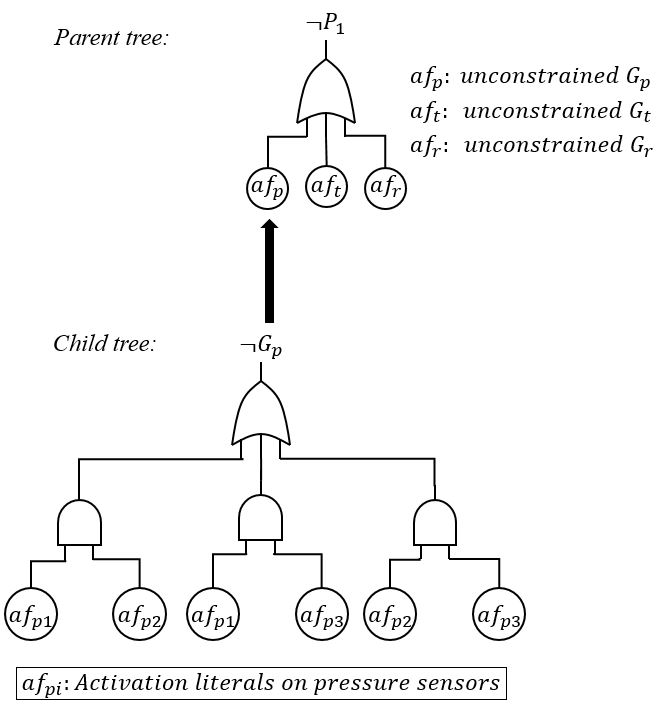
\includegraphics[width=0.5\textwidth]{images/faultCompEx.JPG}
	\end{center}
	\caption{Sensor System Composition of Fault Trees}
	\label{fig:sensorSysComp}
\end{figure}
We return to the sensor system example to illustrate this mapping. Graphically, this is represented in Figure~\ref{fig:sensorSysComp}.  The top level (parent) component is defined as: $\mathit{Comp}_p (M_p, \mathit{FF}_p, \mathit{NFV}_p, \pi_p)$ and $\mathit{FF}_p = \{(\neg P, \mathit{af}_p \lor \mathit{af}_t \lor \mathit{af}_r)\}$ where each activation literal is associated with the unconstrained guarantees $G_p$, $G_t$, and $G_r$. The child layer has a fault forest consisting of three fault trees, one for each subsystem. 

The pressure subsystem fault tree is $\mathit{FT}_{p} = (\neg G_p, (\mathit{af}_{p1} \land \mathit{af}_{p2}) \lor (\mathit{af}_{p1} \land \mathit{af}_{p3}) \lor (\mathit{af}_{p2} \land \mathit{af}_{p3}) $. The leaf formulae for each subsystem tree corresponds to pairwise combinations of active sensor faults. We now show the composition of the pressure subsystem child and top level parent fault trees. 

The mapping $\phi_F$ iterates through each tree in the parent forest -- in this case, we have only one. Then for each parent tree it iterates through the Boolean formulae in $\mathcal{L}$. If there is a match between a child root and a parent leaf, the replacement is made.
Thus, $\mathit{af}_p$ will be replaced with $(\mathit{af}_{p1} \land \mathit{af}_{p2}) \lor (\mathit{af}_{p1} \land \mathit{af}_{p3}) \lor (\mathit{af}_{p2} \land \mathit{af}_{p3})$. This replacement is done for each leaf formula in $\mathcal{L}_p$ from the parent fault forest. 

We represent the unconstrained (violated) guarantee as $\neg G_p$ and it is associated with the fault activation literal $\mathit{af}_p$. The end result of the replacement is easy to see.

%%%%5										COMPOSITION OF FF IS VALID
\begin{lemma} If $\mathit{FF}_c$ and $\mathit{FF}_p$ are valid fault forests, then their composition $\phi(\mathit{FF}_c, \mathit{FF}_p)$ is also a valid fault forest. 
\begin{proof}
By iterative application of Lemma~\ref{lemma:validTree}, the result is immediate.
\end{proof}
\label{lemma:validForest}
\end{lemma}

Thus far, we have proven that a single layer of composition produces valid fault trees (or forests), but to perform this analysis across $n$ layers of architecture we show inductively that the resulting fault forest is valid. 

The notation $\phi_F^n$ indicates the iterated function $\phi_F$ which is a successive application of $\phi_F$ with itself $n$ times. Assume the fault forest $\mathit{FF}_0$ is obtained at the leaf level of the architecture.

\begin{theorem} If $\phi_F^n(\mathit{FF}_{n-1}, \mathit{FF}_n)$ is a valid fault forest, then $\phi^{n+1}(\mathit{FF}_{n}, \mathit{FF}_{n+1})$ is a valid fault forest.
\begin{proof}

Base case: Each fault forest per layer is valid by construction. By Lemma~\ref{lemma:validForest}, $\phi_F(\mathit{FF}_{0}, \mathit{FF}_1)$ is a valid fault forest.

Inductive assumption: Assume $\phi_F^n(\mathit{FF}_{n-1}, \mathit{FF}_n)$ is a valid fault forest.
\begin{equation*}
\begin{split}
\phi_F^{n+1}(\mathit{FF}_{n}, \mathit{FF}_{n+1}) &= ((\mathit{FF}_0 \circ \mathit{FF}_1) \circ \mathit{FF}_2) \circ \cdots \circ \mathit{FF}_n) \circ \mathit{FF}_{n+1})) \\
  &= \phi_F^n(\mathit{FF}_{n-1}, \mathit{FF}_n) \circ \mathit{FF}_{n+1}
\end{split}
\end{equation*}

%$\phi_F^{n+1}(\mathit{FF}_{n}, \mathit{FF}_{n+1}) = ((\mathit{FF}_0 \circ \mathit{FF}_1) \circ \mathit{FF}_2) \circ \cdots \circ \mathit{FF}_n) \circ \mathit{FF}_{n+1})) = \phi_F^n(\mathit{FF}_{n-1}, \mathit{FF}_n) \circ \mathit{FF}_{n+1}$. 

By inductive assumption and Lemma~\ref{lemma:validForest}, $\phi_F^{n+1}(\mathit{FF}_{n}, \mathit{FF}_{n+1})$ is a valid fault forest.

\end{proof}
\label{thm:indForest}
\end{theorem}

We know from previous work that composition is conservative. A valid monolithic analysis of the transition system implies that the compositional analysis of that same system is valid, but the converse may not be true~\cite{}. It is likewise the case for composing fault forests. 

Let $S \subseteq \mathit{AF}$ where all $\mathit{af} \in S$ are constrained to true. If $S \cup \{\neg P\}$ is satisfiable, this equates to a valid fault tree. 

\begin{theorem} If $(I,T) \vdash P$ for monolithic verification, then for $S \subseteq \mathit{AF}$, $S \cup \{\neg P\}$ is unsatisfiable.
\begin{proof}
Assume toward contradiction that $(I,T) \vdash P$ and there exists a set $S \subseteq \mathit{AF}$ such that $S \cup \{\neg P\}$ is satisfiable. This implies that there exists a reachable state such that $\neg P$ holds. This contradicts our assumption. 
\end{proof}
\label{thm:sound}
\end{theorem}

As a counterexample to the converse of Theorem~\ref{thm:sound}, consider the following. \danielle{Counterexample here.}

Now that we have the formal foundations laid, we proceed towards the implementation. 





